% appendices/appendixC.tex
\chapter{Appendix C: Robustness Checks and Supplementary Tests}
\label{appendixC}

This appendix provides detailed results for the robustness checks and supplementary empirical tests discussed in Chapters 5 and 6.

\section{Robustness of Strategic Outsourcing and Wage Pass-Through}

Tables \ref{tab:robustness_outsourcing} and \ref{tab:robustness_wages} present alternative specifications for the two primary reduced-form models. These include excluding outlier states (Manipur), using unweighted averages, and employing different winsorization or categorical treatments of the enforcement variable ($E_s$).

\begin{table}[H]
	\centering
	\caption{Robustness Checks: Strategic Outsourcing (Log Outsourcing Share)}
	\label{tab:robustness_outsourcing}
	
\begingroup
\centering
\begin{tabular}{lccccc}
   \tabularnewline \midrule \midrule
   Dependent Variable: & \multicolumn{5}{c}{ln\_Q\_out}\\
                      & Baseline                     & No Manipur                   & Unweighted                  & Winsor E\_s                 & Quartile E\_s \\    
   Model:             & (1)                          & (2)                          & (3)                         & (4)                         & (5)\\  
   \midrule
   \emph{Variables}\\
   E\_s               & $6.75\times 10^{-6}$         & $5.51\times 10^{-6}$         & $2.17\times 10^{-5}$        & $1.64\times 10^{-6}$        &   \\   
                      & ($1.39\times 10^{-5}$)       & ($1.62\times 10^{-5}$)       & ($3.92\times 10^{-5}$)      & ($1.77\times 10^{-5}$)      &   \\   
   I(I(E\_s\^2))      & $-4.26\times 10^{-6}$        & $-1.82\times 10^{-6}$        & $-1.61\times 10^{-5}$       & $5.76\times 10^{-6}$        &   \\   
                      & ($1.25\times 10^{-5}$)       & ($2.72\times 10^{-5}$)       & ($3.36\times 10^{-5}$)      & ($3.01\times 10^{-5}$)      &   \\   
   ln\_A\_formal      & $3.72\times 10^{-6}$$^{**}$  & $3.73\times 10^{-6}$$^{**}$  & $8.66\times 10^{-6}$$^{*}$  & $3.8\times 10^{-6}$$^{**}$  & $3.69\times 10^{-6}$$^{**}$\\    
                      & ($1.74\times 10^{-6}$)       & ($1.75\times 10^{-6}$)       & ($4.51\times 10^{-6}$)      & ($1.74\times 10^{-6}$)      & ($1.77\times 10^{-6}$)\\    
   E\_s\_QQ2          &                              &                              &                             &                             & $6.24\times 10^{-7}$\\    
                      &                              &                              &                             &                             & ($3.99\times 10^{-6}$)\\    
   E\_s\_QQ3          &                              &                              &                             &                             & $-1.4\times 10^{-6}$\\    
                      &                              &                              &                             &                             & ($3.02\times 10^{-6}$)\\    
   E\_s\_QQ4\_high    &                              &                              &                             &                             & $2.18\times 10^{-6}$\\    
                      &                              &                              &                             &                             & ($3.57\times 10^{-6}$)\\    
   \midrule
   \emph{Fixed-effects}\\
   NIC\_2digit        & Yes                          & Yes                          & Yes                         & Yes                         & Yes\\  
   \midrule
   \emph{Fit statistics}\\
   Observations       & 47                           & 46                           & 47                          & 47                          & 47\\  
   R$^2$              & 0.12204                      & 0.11804                      & 0.09281                     & 0.12320                     & 0.13248\\  
   Within R$^2$       & 0.10169                      & 0.09968                      & 0.08646                     & 0.10288                     & 0.11238\\  
   \midrule \midrule
   \multicolumn{6}{l}{\emph{Clustered (State\_Code) standard-errors in parentheses}}\\
   \multicolumn{6}{l}{\emph{Signif. Codes: ***: 0.01, **: 0.05, *: 0.1}}\\
\end{tabular}
\par\endgroup



\end{table}

\begin{table}[H]
	\centering
	\caption{Robustness Checks: Wage Pass-Through (Log Informal Wage)}
	\label{tab:robustness_wages}
	
\begingroup
\centering
\begin{tabular}{lccccc}
   \tabularnewline \midrule \midrule
   Dependent Variable: & \multicolumn{5}{c}{ln\_w\_inf}\\
                                   & Baseline & No Manipur & Unweighted & Winsor E\_s  & Quartile E\_s \\    
   Model:                          & (1)      & (2)        & (3)        & (4)          & (5)\\  
   \midrule
   \emph{Variables}\\
   E\_s                            & 0.1140   & 6.293      & 0.9010     & 1.159        &   \\   
                                   & (5.087)  & (4.808)    & (5.350)    & (6.421)      &   \\   
   ln\_A\_formal                   & -0.0286  & 0.0248     & -0.0034    & -0.0051      & -0.0258\\   
                                   & (0.0715) & (0.0643)   & (0.0764)   & (0.0696)     & (0.0723)\\   
   E\_s $\times$ ln\_A\_formal     & -0.0592  & -0.4847    & -0.1042    & -0.1311      &   \\   
                                   & (0.3784) & (0.3618)   & (0.4181)   & (0.4664)     &   \\   
   E\_s\_QQ2                       &          &            &            &              & -0.0457\\   
                                   &          &            &            &              & (0.1481)\\   
   E\_s\_QQ3                       &          &            &            &              & -0.0993\\   
                                   &          &            &            &              & (0.2336)\\   
   E\_s\_QQ4\_high                 &          &            &            &              & -0.2342\\   
                                   &          &            &            &              & (0.1999)\\   
   \midrule
   \emph{Fixed-effects}\\
   NIC\_2digit                     & Yes      & Yes        & Yes        & Yes          & Yes\\  
   \midrule
   \emph{Fit statistics}\\
   Observations                    & 47       & 46         & 47         & 47           & 47\\  
   R$^2$                           & 0.09587  & 0.05406    & 0.05523    & 0.06368      & 0.05114\\  
   Within R$^2$                    & 0.08139  & 0.04743    & 0.04723    & 0.04869      & 0.03595\\  
   \midrule \midrule
   \multicolumn{6}{l}{\emph{Clustered (State\_Code) standard-errors in parentheses}}\\
   \multicolumn{6}{l}{\emph{Signif. Codes: ***: 0.01, **: 0.05, *: 0.1}}\\
\end{tabular}
\par\endgroup



\end{table}

\newpage
\section{Alternative Enforcement and Heterogeneity}

Table \ref{tab:alt_enforcement} uses an alternative measure of enforcement: the number of factory inspectors per 1,000 working factories. Table \ref{tab:heterogeneity} explores how the main results vary across the Textiles and Apparel sub-sectors and by the overall level of state enforcement.

\begin{table}[H]
	\centering
	\caption{Alternative Enforcement: Inspectors per Factory}
	\label{tab:alt_enforcement}
	
\begingroup
\centering
\begin{tabular}{lcc}
   \tabularnewline \midrule \midrule
   Dependent Variables:                  & ln\_w\_inf   & ln\_Q\_out\\    
                                         & Wages        & Outsourcing \\   
   Model:                                & (1)          & (2)\\  
   \midrule
   \emph{Variables}\\
   E\_s\_alt                             & 40.94        & -0.0001\\   
                                         & (72.38)      & (0.0002)\\   
   ln\_A\_formal                         & 0.0512       & $3.46\times 10^{-6}$\\    
                                         & (0.0875)     & ($2.16\times 10^{-6}$)\\    
   E\_s\_alt $\times$ ln\_A\_formal      & -3.207       &   \\   
                                         & (5.865)      &   \\   
   I(I(E\_s\_alt\^2))                    &              & 0.0003\\   
                                         &              & (0.0005)\\   
   \midrule
   \emph{Fixed-effects}\\
   NIC\_2digit                           & Yes          & Yes\\  
   \midrule
   \emph{Fit statistics}\\
   Observations                          & 45           & 45\\  
   R$^2$                                 & 0.06132      & 0.12773\\  
   Within R$^2$                          & 0.05087      & 0.10434\\  
   \midrule \midrule
   \multicolumn{3}{l}{\emph{Clustered (State\_Code) standard-errors in parentheses}}\\
   \multicolumn{3}{l}{\emph{Signif. Codes: ***: 0.01, **: 0.05, *: 0.1}}\\
\end{tabular}
\par\endgroup



\end{table}

\begin{table}[H]
	\centering
	\caption{Heterogeneity Analysis: Industry and Enforcement Splits}
	\label{tab:heterogeneity}
	
\begingroup
\centering
\begin{tabular}{lcccc}
   \tabularnewline \midrule \midrule
   Dependent Variable: & \multicolumn{4}{c}{ln\_Q\_out}\\
                   & Textiles                & Apparel                     & High E\_s                  & Low E\_s \\    
   Model:          & (1)                     & (2)                         & (3)                        & (4)\\  
   \midrule
   \emph{Variables}\\
   Constant        & $-3.54\times 10^{-5}$   & $-8.5\times 10^{-5}$$^{*}$  &                            &   \\   
                   & ($2.61\times 10^{-5}$)  & ($4.19\times 10^{-5}$)      &                            &   \\   
   E\_s            & $1.4\times 10^{-5}$     & $2.82\times 10^{-5}$        &                            &   \\   
                   & ($2.61\times 10^{-5}$)  & ($3.32\times 10^{-5}$)      &                            &   \\   
   I(I(E\_s\^2))   & $-1\times 10^{-5}$      & $-4.65\times 10^{-5}$       &                            &   \\   
                   & ($2.09\times 10^{-5}$)  & ($4.44\times 10^{-5}$)      &                            &   \\   
   ln\_A\_formal   & $2.61\times 10^{-6}$    & $6.46\times 10^{-6}$$^{*}$  & $7\times 10^{-6}$$^{***}$  & $1.6\times 10^{-6}$\\    
                   & ($1.99\times 10^{-6}$)  & ($3.29\times 10^{-6}$)      & ($2.23\times 10^{-6}$)     & ($1.12\times 10^{-6}$)\\    
   \midrule
   \emph{Fixed-effects}\\
   NIC\_2digit     &                         &                             & Yes                        & Yes\\  
   \midrule
   \emph{Fit statistics}\\
   Observations    & 25                      & 22                          & 22                         & 25\\  
   R$^2$           & 0.14162                 & 0.13332                     & 0.30914                    & 0.09312\\  
   Within R$^2$    &                         &                             & 0.30908                    & 0.02030\\  
   \midrule \midrule
   \multicolumn{5}{l}{\emph{Clustered (State\_Code) standard-errors in parentheses}}\\
   \multicolumn{5}{l}{\emph{Signif. Codes: ***: 0.01, **: 0.05, *: 0.1}}\\
\end{tabular}
\par\endgroup



\end{table}

\newpage
\section{Diagnostic Checks: Placebo and Outliers}

As discussed in Section 5.3, the placebo test in the Chemicals sector (NIC-20) confirms that the productivity-outsourcing relationship is specific to labor-intensive manufacturing. Figure \ref{fig:outlier_diag} identifies influential observations in the wage pass-through model.

\begin{table}[H]
	\centering
	\caption{Placebo Test: Chemicals Sector (NIC-20)}
	\label{tab:placebo}
	
\begingroup
\centering
\begin{tabular}{lc}
   \tabularnewline \midrule \midrule
   Dependent Variable: & ln\_Q\_out\\    
   Model:              & (1)\\  
   \midrule
   \emph{Variables}\\
   ln\_A\_formal       & -0.0009\\   
                       & (0.0047)\\   
   E\_s                & 0.0013\\   
                       & (0.0152)\\   
   \midrule
   \emph{Fixed-effects}\\
   NIC\_2digit         & Yes\\  
   \midrule
   \emph{Fit statistics}\\
   Observations        & 27\\  
   R$^2$               & 0.00015\\  
   Within R$^2$        & 0.00015\\  
   \midrule \midrule
   \multicolumn{2}{l}{\emph{Clustered (State\_Code) standard-errors in parentheses}}\\
   \multicolumn{2}{l}{\emph{Signif. Codes: ***: 0.01, **: 0.05, *: 0.1}}\\
\end{tabular}
\par\endgroup



\end{table}

\begin{figure}[H]
	\centering
	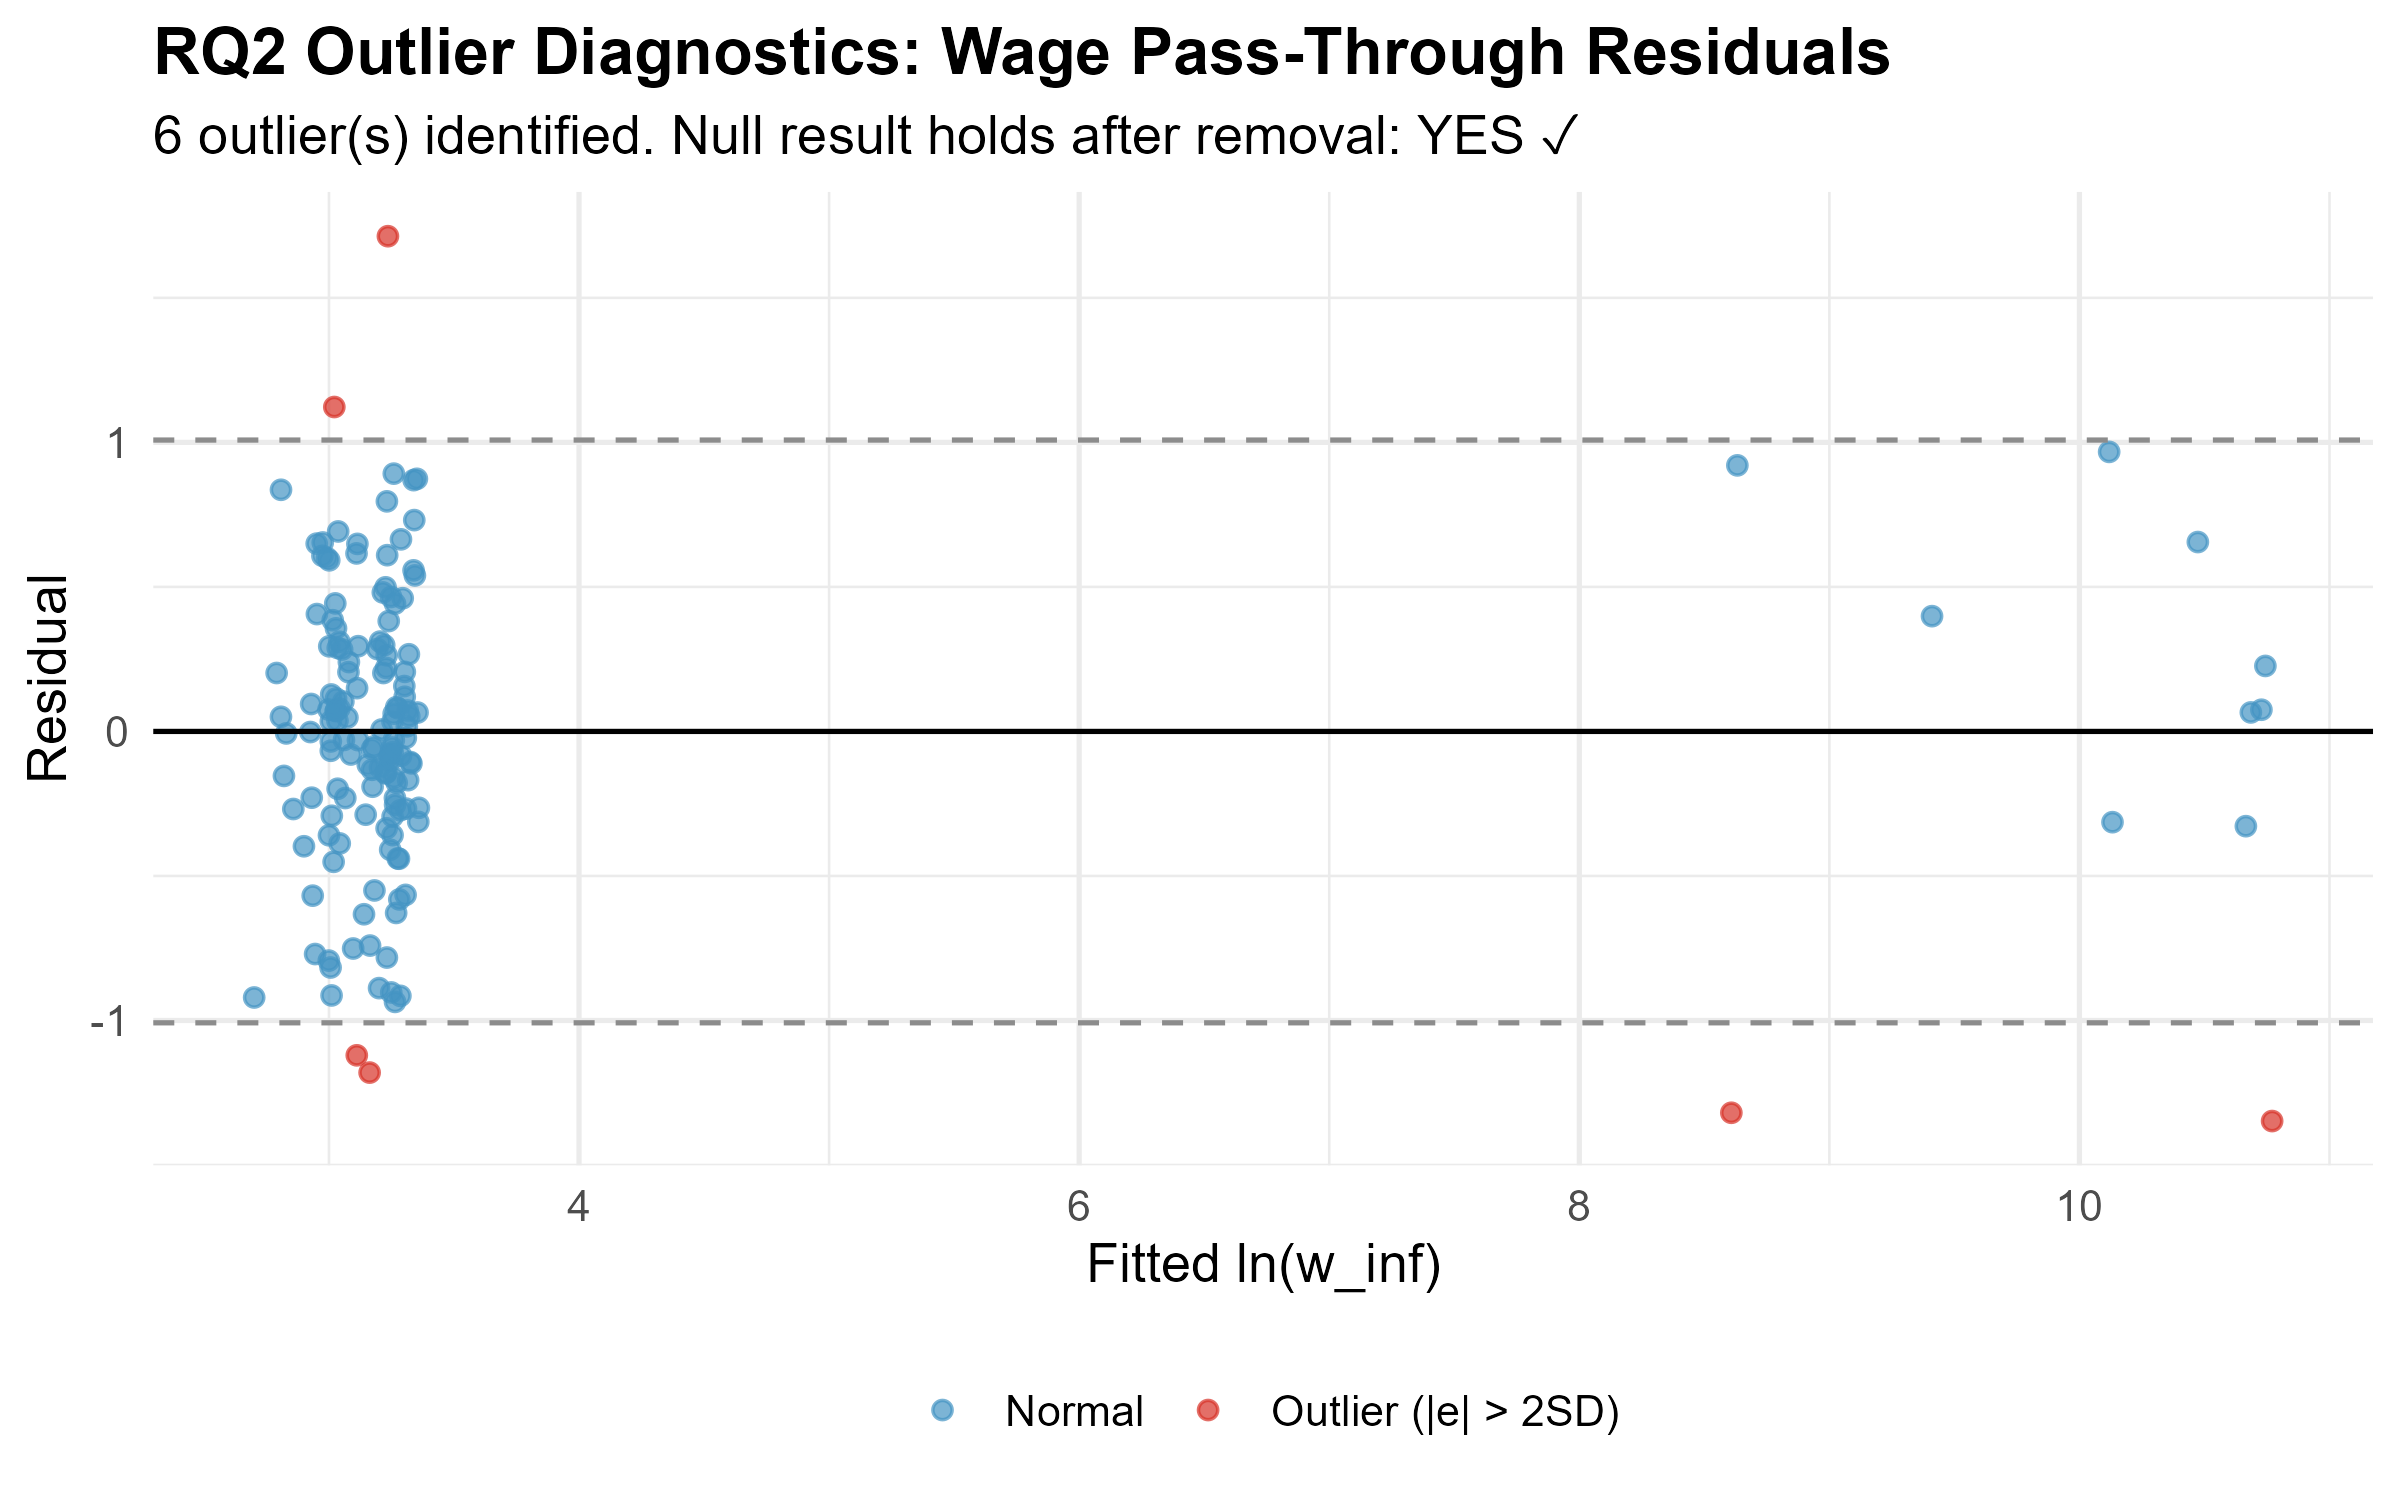
\includegraphics[width=0.85\textwidth]{../Output/images/figure_robustness_rq2_outliers}
	\caption{Outlier Diagnostics: Wage Pass-Through Residuals}
	\label{fig:outlier_diag}
\end{figure}

\newpage
\section{Supplementary Political Economy Tests}

The following tables provide the results for the supplementary tests described in Chapter 6, covering asymmetric cost structures, firm size effects, and market concentration.

\begin{table}[H]
	\centering
	\caption{Supplementary Test 4: Asymmetric Cost Shifting}
	\label{tab:supp_test4}
	
\begingroup
\centering
\begin{tabular}{lc}
   \tabularnewline \midrule \midrule
   Dependent Variable:                        & delta\_w\_inf\\    
   Model:                                     & (1)\\  
   \midrule
   \emph{Variables}\\
   E\_s                                       & 0.6308\\   
                                              & (0.4483)\\   
   delta\_A\_formal $\times$ A\_increases     & -0.0105\\   
                                              & (0.2756)\\   
   delta\_A\_formal $\times$ A\_decreases     & 1.376\\   
                                              & (1.323)\\   
   \midrule
   \emph{Fixed-effects}\\
   NIC\_2digit                                & Yes\\  
   Year                                       & Yes\\  
   \midrule
   \emph{Fit statistics}\\
   Observations                               & 101\\  
   R$^2$                                      & 0.73105\\  
   Within R$^2$                               & 0.11607\\  
   \midrule \midrule
   \multicolumn{2}{l}{\emph{Clustered (State\_Code) standard-errors in parentheses}}\\
   \multicolumn{2}{l}{\emph{Signif. Codes: ***: 0.01, **: 0.05, *: 0.1}}\\
\end{tabular}
\par\endgroup



\end{table}

\begin{table}[H]
	\centering
	\caption{Supplementary Test 5: Firm Size and Informality Scale}
	\label{tab:supp_test5}
	
\begingroup
\centering
\begin{tabular}{lcc}
   \tabularnewline \midrule \midrule
   Dependent Variables:                       & ln\_Q\_out   & ln\_w\_inf\\    
   Model:                                     & (1)          & (2)\\  
   \midrule
   \emph{Variables}\\
   ln\_firm\_size                             & 0.0140       & -0.6739\\   
                                              & (0.0206)     & (1.429)\\   
   ln\_A\_formal                              & 0.0126       & 0.2334\\   
                                              & (0.0101)     & (0.5281)\\   
   E\_s                                       & 0.0373       & 1.584\\   
                                              & (0.0263)     & (1.601)\\   
   ln\_firm\_size $\times$ ln\_A\_formal      & -0.0012      & 0.0403\\   
                                              & (0.0015)     & (0.1056)\\   
   \midrule
   \emph{Fixed-effects}\\
   NIC\_2digit                                & Yes          & Yes\\  
   \midrule
   \emph{Fit statistics}\\
   Observations                               & 152          & 152\\  
   R$^2$                                      & 0.25386      & 0.13347\\  
   Within R$^2$                               & 0.24803      & 0.13196\\  
   \midrule \midrule
   \multicolumn{3}{l}{\emph{Clustered (State\_Code) standard-errors in parentheses}}\\
   \multicolumn{3}{l}{\emph{Signif. Codes: ***: 0.01, **: 0.05, *: 0.1}}\\
\end{tabular}
\par\endgroup



\end{table}

\begin{table}[H]
	\centering
	\caption{Supplementary Test 7: Employment Threshold Effects}
	\label{tab:supp_test7}
	
\begingroup
\centering
\begin{tabular}{lc}
   \tabularnewline \midrule \midrule
   Dependent Variable:                              & ln\_w\_inf\\    
   Model:                                           & (1)\\  
   \midrule
   \emph{Variables}\\
   E\_s                                             & 3.736$^{*}$\\   
                                                    & (1.863)\\   
   ln\_A\_formal $\times$ as.integer(E\_s>=0.3)     & 0.8325$^{**}$\\   
                                                    & (0.3244)\\   
   ln\_A\_formal $\times$ as.integer(E\_s<0.3)      & 0.9186$^{**}$\\   
                                                    & (0.3352)\\   
   \midrule
   \emph{Fixed-effects}\\
   NIC\_2digit                                      & Yes\\  
   \midrule
   \emph{Fit statistics}\\
   Observations                                     & 152\\  
   R$^2$                                            & 0.25002\\  
   Within R$^2$                                     & 0.24871\\  
   \midrule \midrule
   \multicolumn{2}{l}{\emph{Clustered (State\_Code) standard-errors in parentheses}}\\
   \multicolumn{2}{l}{\emph{Signif. Codes: ***: 0.01, **: 0.05, *: 0.1}}\\
\end{tabular}
\par\endgroup



\end{table}

\begin{table}[H]
	\centering
	\caption{Supplementary Test 8: Market Concentration and Monopsony}
	\label{tab:supp_test8}
	
\begingroup
\centering
\begin{tabular}{lcc}
   \tabularnewline \midrule \midrule
   Dependent Variable: & \multicolumn{2}{c}{ln\_w\_inf}\\
   Model:                                       & (1)           & (2)\\  
   \midrule
   \emph{Variables}\\
   ln\_concentration                            & 0.0217        & 3.168$^{**}$\\   
                                                & (0.0946)      & (1.512)\\   
   ln\_A\_formal                                & 0.9749$^{**}$ & 0.2473\\   
                                                & (0.3758)      & (0.3207)\\   
   E\_s                                         & 2.034         & 1.386\\   
                                                & (1.262)       & (1.223)\\   
   ln\_concentration $\times$ ln\_A\_formal     &               & -0.2288$^{*}$\\   
                                                &               & (0.1118)\\   
   \midrule
   \emph{Fixed-effects}\\
   NIC\_2digit                                  & Yes           & Yes\\  
   \midrule
   \emph{Fit statistics}\\
   Observations                                 & 152           & 152\\  
   R$^2$                                        & 0.22083       & 0.25351\\  
   Within R$^2$                                 & 0.21947       & 0.25221\\  
   \midrule \midrule
   \multicolumn{3}{l}{\emph{Clustered (State\_Code) standard-errors in parentheses}}\\
   \multicolumn{3}{l}{\emph{Signif. Codes: ***: 0.01, **: 0.05, *: 0.1}}\\
\end{tabular}
\par\endgroup



\end{table}
